\documentclass[11pt,aspectratio=1610,dvipsnames]{beamer}
\graphicspath{{figs/}}
\usetheme{default}
\usepackage{DasBeamerPaket}
\usepackage{animate}
\usepackage{lastpage}
\usepackage{tikz}
\usepackage{lmodern}
\setbeamercolor{section in toc}{fg=NavyBlue}
\setbeamercolor{frametitle}{fg=NavyBlue}
\captionsetup[figure]{labelfont=bf}
\captionsetup[table]{labelfont=bf}
\setbeamertemplate{caption}[numbered]
\title[$\Lambda(1405)$]{Experimental studies of the $\Lambda(1405)$}
\subtitle[Seminar physics654]{physics654 -- Seminar on exotic multi-quark states}

\begin{document}
\definecolor{myWhite}{rgb}{1,1,1}

\setbeamertemplate{footline}[text line]{\parbox{0.3\linewidth}{\vspace*{-9pt}\textcolor{white} \insertsection  \hfill} \parbox{0.7\linewidth}{\vspace*{-8pt} \textcolor{white}{\hfill\hspace{-3cm}\insertshorttitle \phantom{ }-- \insertshortsubtitle}  \hfill \textcolor{myWhite}{\insertpagenumber/\pageref{LastPage}}}}

\addtobeamertemplate{footline}{ \makebox[0pt][l]{\hspace{-1cm}
		\raisebox{0cm}[0pt][0pt]{\colorbox{gray!20!black}{\phantom{{\large TEXTTEXTTEXTTEXTTEXTTEXTTEXTTEXTTEXTTEXTTEXTTEXTTEXTTEXTTEXTTEXTTEXTTEXTTEXTTEXTTEXTTEXTTEXTTEXTTEXTTEXTTEXTTEXTTEXTTEXTTEXTTEXTTEXTTEXTTEXTTEXTTEXTTEXTTEXTTEXT}}}}}}

\setbeamercovered{transparent}
\setbeamertemplate{navigation symbols}{}
\setbeamertemplate{frametitle}[default][left,leftskip=0.5cm]
%
\setbeamertemplate{itemize item}{\color{black}$\blacktriangleright$}
\setbeamertemplate{section in toc}[sections numbered]
\captionsetup{font=scriptsize,labelfont=scriptsize}

\AtBeginSection[]
{	
	\definecolor{myWhite}{rgb}{0,0,0}
	\begin{frame}[noframenumbering]
		\frametitle{}
		\addtocounter{page}{-1}
		\tableofcontents[currentsection]
		
	\end{frame}
\definecolor{myWhite}{rgb}{1,1,1}
}


\begin{frame}[plain]
	\setcounter{page}{0}
	\centering
	{\Large \color{MidnightBlue}{Experimental studies of the $\Lambda(1405)$}}\\
	{\href{https://www.youtube.com/watch?v=oHg5SJYRHA0}{physics654 -- Seminar on exotic multi-quark states}}
	

	\vfill

		



			
	\textsc{Jakob Krause}\\
	\scriptsize \href{mailto:krause@hiskp.uni-bonn.de}{\faEnvelope  \hspace*{0.1cm}krause@hiskp.uni-bonn.de} {\color{black}$|$} \href{https://github.com/krausejm}{\faGithub  \hspace*{0.1cm}krausejm}\\
	
	\vspace{.5cm}
	
	Tutor: \textsc{Georg Scheluchin}\\
	 \href{mailto:scheluchin@physik.uni-bonn.de}{\faEnvelope  \hspace*{0.1cm}scheluchin@physik.uni-bonn.de}

	\vspace{0.2cm}
	
	18.06.2021
	 	
 		
\end{frame}
\section*{Motivation}
\begin{frame}{Motivation}
\begin{minipage}{\linewidth}
		\begin{tcolorbox}[colback=black!10,colframe=gray!20!black,title=What is special about the $\Lambda(1405)$?] 
			\begin{itemize}
				\item its mass does not fit well into constituent quark models which do predict baryon masses well for other baryons 
				\item invariant mass distribution (line shape) differs significantly from usual \textsc{Breit-Wigner} shapes
				\item candidate for an exotic multiquark state (bound system of $\overline{K}N$) since its mass lies just below threshold
			
 			\end{itemize}
 		\vspace{.5cm}
 		There are (very) many different theoretical approaches to explain this behavior\\
 		$\to$ There is need for more experimental data!
		\end{tcolorbox}
	{\color{red} some plots/pictures?}
\end{minipage}




	
\end{frame}
%\begin{frame}[plain]
%	\maketitle
%	\setcounter{page}{0}
%\end{frame}
\section*{Table of contents}
\begin{frame}{Table of contents}
	\tableofcontents
\end{frame}
\section{Experimental setup}
\begin{frame}{Continuous Electron Beam Accelerator Facility (CEBAF)}
	\begin{figure}
		\centering
		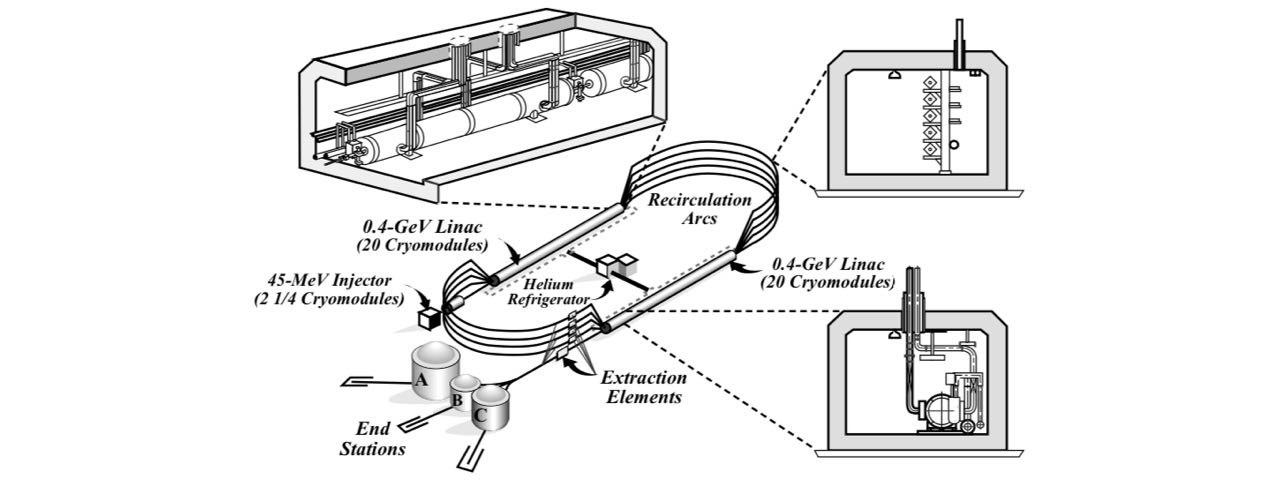
\includegraphics[width=\linewidth]{setup_big.jpg}
		\caption{CEBAF layout at Jefferson Lab, [\cite{clas}]}
	\end{figure}
\end{frame}
\begin{frame}{CEBAF Large Acceptance Spectrometer (CLAS)}
	\begin{figure}
		\centering
		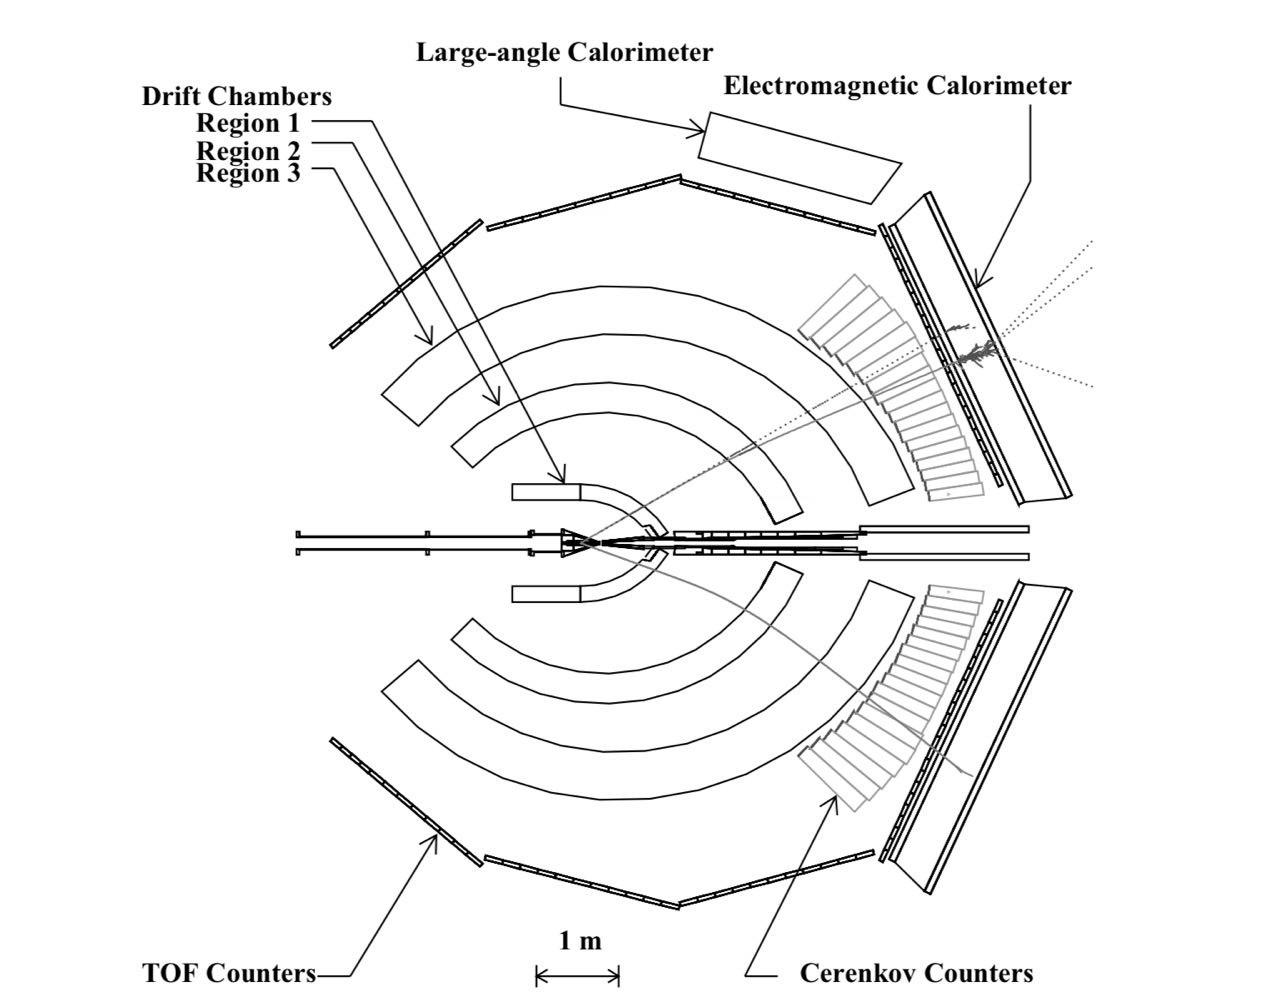
\includegraphics[width=.7\linewidth]{setup.jpg}
		\caption{CLAS layout at Jefferson Lab, [\cite{clas}]}
	\end{figure}
\end{frame}

\section{Spin-parity measurement}

\section{Line-shape measurement}

\section{Conclusion}








\end{document}